	\chapter*{Annexe A2 : Utilisation de CART dans la construction des Forêts aléatoires}
En comparaison avec le modèle CART qui lui procède à une phase de construction de l'arbre suivie d'une phase d'élagage, deux différences sont à relever. D'abord, à chaque nœud, un nombre paramètre (dénoté \textit{k}\footnote{L'autre paramètre des FA étant \textit{B}, le nombre d'arbres dont la forêt.}) de variables exogènes sont choisies aléatoirement et la meilleure variable pour la subdivision du nœud est choisie parmi celles-ci seulement. Ensuite, aucun élagage n'est introduit: tous les arbres de la forêt sont maximaux.\par
	Le principe de CART est de partitionner récursivement l’espace engendré par les variables explicatives (ici $\reels^p$) de façon dyadique. Plus précisément, à
	chaque étape du partitionnement, on découpe une partie de l’espace en deux sous parties selon une variable $X_j$ comme le montre la figure \ref{fig:CART}.
	\begin{figure}[h]
	    		\centering
	    		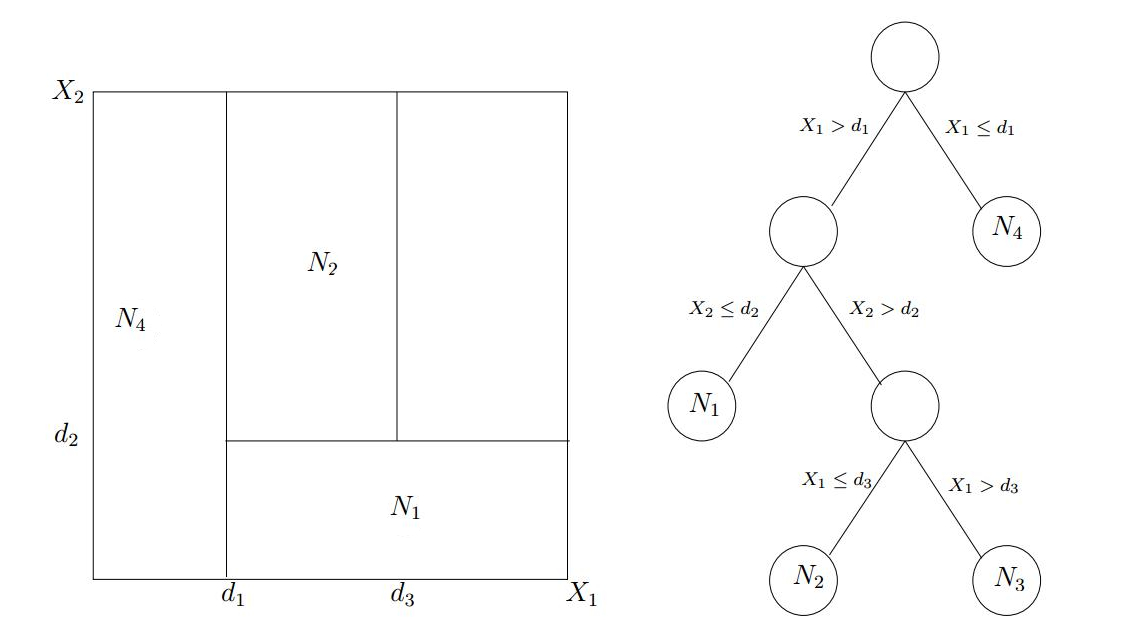
\includegraphics[scale=0.35]{Cart}
	    		\caption{Arbre CART}
	    		\label{fig:CART}
	\end{figure}
	\par
	Les coupures sont choisies de manière à minimiser une fonction de coût particulière. A chaque étape, on cherche la variable $X_j$ et le réel \textit{d} qui minimisent la variance des nœuds fils dans les problèmes de régression. Les arbres sont ainsi construits jusqu’à atteindre une règle d’arrêt. Par exemple, on ne découpe pas un nœud qui contient moins de 5 observations comme y procède le package \textbf{\textit{randomForest}} du langage \textbf{R}.\par
	L'agrégation à laquelle procèdent les FA est d’autant plus performante que la corrélation entre les prédicteurs agrégés  (arbres CART) est faible. Afin de diminuer cette corrélation, Breiman\cite{BREI01} propose de rajouter une couche d’aléa dans la construction des
		prédicteurs. Plus précisément, à chaque étape de CART, \textit{k} variables sont sélectionnées aléatoirement parmi les \textit{p} et la meilleure coupure est sélectionnée uniquement sur ces \textit{k} variables. \par
		On retrouve un compromis biais-variance dans le choix de m :
		\begin{itemize}
		\item lorsque \textit{k} diminue, la tendance est à se rapprocher d’un choix aléatoire des variables
		de découpe des arbres. Dans le cas extrême où \textit{k} = 1, les axes de la partition des arbres
		sont choisies au hasard, seuls les points de coupure utiliseront l’échantillon. Ainsi, si \textit{k}
		diminue, la corrélation entre les arbres va avoir tendance à diminuer également, ce qui
		entraînera une baisse de la variance de l’estimateur agrégé. En revanche, choisir les axes
		de découpe des arbres de manière aléatoire va se traduire par une moins bonne
		qualité d’ajustement des arbres sur l’échantillon d’apprentissage, d’où une augmentation
		du biais pour chaque arbre ainsi que pour l’estimateur agrégé.
		\item lorsque \textit{k} augmente, les phénomènes inverses se produisent.
		\end{itemize}
		On déduit de cette remarque que le choix de \textit{k} est lié aux choix des paramètres de l’arbre,
		notamment au choix du nombre d’observations dans ses nœuds terminaux. En effet, si ce
		nombre est petit, chaque arbre aura un biais faible mais une forte variance. Il faudra dans ce cas là s’attacher à diminuer cette variance et on aura donc plutôt tendance à choisir une
		valeur de \textit{k} relativement faible. A l’inverse, si les arbres ont un grand nombre d’observations
		dans leurs nœuds terminaux, ils posséderont moins de variance mais un biais plus élevé. Dans
		ce cas, la procédure d’agrégation se révélera moins efficace. C’est pourquoi, en pratique, le
		nombre maximum d’observations dans les nœuds est par défaut pris relativement petit (5). Concernant le choix de \textit{k}, \textit{\textbf{randomForest}} propose par
		défaut \textit{k = $\frac{p}{3}$} en régression. Ce paramètre peut également
		être sélectionné via des procédures apprentissage-validation ou validation croisée.